\documentclass[border=7pt]{standalone}
\usepackage{fontspec,unicode-math}
\setmainfont{Noto Serif}
\setmathfont{STIXTwoMath-Regular.otf}
\usepackage{tikz}
\usetikzlibrary{arrows.meta,calc,patterns,decorations.markings,decorations.pathmorphing,decorations.pathreplacing}
\tikzset{lev/.style={line width=1.1pt,line cap=butt},
 fine/.style={line width=.52pt},light/.style={line width=.35pt},
 curve/.style={line width=1.15pt,line cap=round,line join=round},
 ax/.style={line width=.57pt,-{Latex[length=2mm,width=1.15mm]}},
 ray/.style={line width=.58pt,-{Latex[length=1.9mm,width=1mm]},shorten >=1.2pt,shorten <=1.2pt},
 dim/.style={line width=.50pt,{Latex[length=1.65mm,width=.85mm]}-{Latex[length=1.65mm,width=.85mm]}},
 flow/.style={line width=.65pt,postaction={decorate},decoration={markings,mark=at position .6 with {\arrow{Latex[length=1.8mm,width=.95mm]}}}},
 lab/.style={font=\fontsize{12}{14.4}\selectfont,inner sep=1.5pt},
 small/.style={font=\fontsize{10.5}{12.5}\selectfont,inner sep=1.2pt},
 panel/.style={font=\fontsize{12}{14.4}\selectfont\itshape,inner sep=1.5pt}}
\pagestyle{empty}
\begin{document}
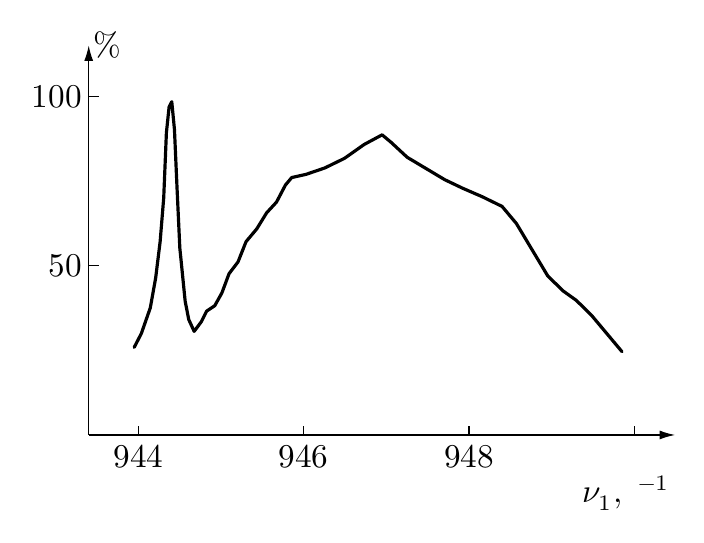
\begin{tikzpicture}[x=1cm,y=1cm,line join=round]
\draw[ax] (0,0)--(7.45,0) node[lab,below left,yshift=-13pt] {$\nu_1,\ \mathrm{см}^{-1}$};
\draw[ax] (0,0)--(0,4.95) node[lab,right] {$\%$};
\draw[fine] (0.63000,0)--++(0,.12);\node[lab,below] at (0.63000,-.07) {$ 944 $};
\draw[fine] (2.73000,0)--++(0,.12);\node[lab,below] at (2.73000,-.07) {$ 946 $};
\draw[fine] (4.83000,0)--++(0,.12);\node[lab,below] at (4.83000,-.07) {$ 948 $};
\draw[fine] (0,2.15000)--++(.13,0);\node[lab,left] at (-.03,2.15000) {$ 50 $};
\draw[fine] (0,4.30000)--++(.13,0);\node[lab,left] at (-.03,4.30000) {$ 100 $};
\draw[fine] (6.93000,0)--++(0,.12);
% CP10: source-guided hand trace (47 visible bends) of the PRINTED curve.
% The points are graphical anchors, NOT independent experimental observations.
% No smoothing or invented measurement markers.
\draw[curve] plot coordinates {(0.57750,1.11230) (0.66844,1.28864) (0.78211,1.61420) (0.85031,1.99401) (0.90714,2.45521) (0.95261,3.01136) (0.98671,3.83880) (1.02081,4.16435) (1.05491,4.23218) (1.08901,3.87950) (1.12311,3.10631) (1.15722,2.37382) (1.22542,1.69558) (1.27089,1.46498) (1.33909,1.31577) (1.43002,1.43785) (1.49822,1.57350) (1.60053,1.64132) (1.69146,1.80410) (1.78240,2.04826) (1.89607,2.19748) (1.99837,2.45521) (2.13478,2.61798) (2.25981,2.82145) (2.38485,2.95710) (2.49852,3.17413) (2.57809,3.26909) (2.75996,3.30978) (2.99867,3.39117) (3.24874,3.51325) (3.49881,3.68959) (3.72615,3.81167) (3.83982,3.71672) (4.04443,3.52681) (4.24903,3.40473) (4.52184,3.24196) (4.74918,3.13344) (4.99925,3.02492) (5.24933,2.90284) (5.43120,2.68580) (5.65854,2.30599) (5.82904,2.02114) (6.02228,1.83123) (6.19278,1.70915) (6.38602,1.51924) (6.54516,1.32934) (6.77250,1.05804)};

\end{tikzpicture}
\end{document}
